% =============================================================================
% COPYRIGHT AND DISCLAIMER
% =============================================================================
% This file is provided as a convenience template for competition participants.
% By using it, you accept full responsibility for compliance with all applicable
% copyright, licensing, and usage rules of the Association for Computing
% Machinery (ACM) and of any LaTeX packages you load (including, without
% limitation, the "acmart" document class and related ACM materials).
%
% Consult ACM's official publication, template, and copyright policies before
% using this setup for any purpose other than this competition. Do not assume
% that this template may be reused, redistributed, or submitted elsewhere
% without independently verifying ACM's current rules.
%
% Use of the "acmart" class, the "sigconf" option, or ACM-style formatting in
% this template does NOT mean that this report, this competition, its organizers,
% or any resulting PDF is sponsored, endorsed, affiliated with, or published by
% ACM. ACM trademarks and branding remain the property of ACM.
%
% Template packages live in preamble.tex.
% Citations live in main.bib. Edit this file with your paper content.
% =============================================================================

\documentclass[sigconf]{acmart}
% =============================================================================
% Template setup — participants normally do not edit this file.
% Author content belongs in main.tex; citations belong in main.bib.
% \documentclass lives in main.tex so Overleaf does not treat this file as root.
% =============================================================================

% --- Competition / non-ACM-submission friendly rights metadata -------------
\setcopyright{none}
\settopmatter{printacmref=false}
\acmConference[Kaggle Competition]{Filament Segmentation Challenge}{2026}{\href{https://www.kaggle.com/competitions/filament-segmentation-2026}{kaggle.com/competitions/filament-segmentation-2026}}
\acmBooktitle{Competition Report}
\acmDOI{}
\acmISBN{}

% --- Author guidance text --------------------------------------------------
% \guide{...} is gray italic while \guideStyletrue; omitted from the PDF if false.
% Flip the switch in main.tex after % =============================================================================
% Template setup — participants normally do not edit this file.
% Author content belongs in main.tex; citations belong in main.bib.
% \documentclass lives in main.tex so Overleaf does not treat this file as root.
% =============================================================================

% --- Competition / non-ACM-submission friendly rights metadata -------------
\setcopyright{none}
\settopmatter{printacmref=false}
\acmConference[Kaggle Competition]{Filament Segmentation Challenge}{2026}{\href{https://www.kaggle.com/competitions/filament-segmentation-2026}{kaggle.com/competitions/filament-segmentation-2026}}
\acmBooktitle{Competition Report}
\acmDOI{}
\acmISBN{}

% --- Author guidance text --------------------------------------------------
% \guide{...} is gray italic while \guideStyletrue; omitted from the PDF if false.
% Flip the switch in main.tex after % =============================================================================
% Template setup — participants normally do not edit this file.
% Author content belongs in main.tex; citations belong in main.bib.
% \documentclass lives in main.tex so Overleaf does not treat this file as root.
% =============================================================================

% --- Competition / non-ACM-submission friendly rights metadata -------------
\setcopyright{none}
\settopmatter{printacmref=false}
\acmConference[Kaggle Competition]{Filament Segmentation Challenge}{2026}{\href{https://www.kaggle.com/competitions/filament-segmentation-2026}{kaggle.com/competitions/filament-segmentation-2026}}
\acmBooktitle{Competition Report}
\acmDOI{}
\acmISBN{}

% --- Author guidance text --------------------------------------------------
% \guide{...} is gray italic while \guideStyletrue; omitted from the PDF if false.
% Flip the switch in main.tex after \input{preamble}.
%
% Do not use \guide{...} for \email{...}.
\usepackage{xcolor}
\newif\ifguideStyle
\guideStyletrue
\newcommand{\guide}[1]{%
  \ifguideStyle
    {\color{gray!65}\itshape #1}%
  \fi
}

% --- Math ------------------------------------------------------------------
% Do NOT load amssymb (or amsfonts): acmart already loads newtxmath, which
% defines the same symbols (e.g. \Bbbk) and causes a conflict on Overleaf.
% amsmath is already provided by acmart; mathtools extends it.
\usepackage{mathtools}

% --- Figures ---------------------------------------------------------------
% graphicx is already loaded by acmart
\usepackage{subcaption}

% --- Tables ----------------------------------------------------------------
% booktabs is already loaded by acmart
\usepackage{tabularx}
\usepackage{multirow}

% --- Bibliography style is set in main.tex (ACM-Reference-Format) ----------
.
%
% Do not use \guide{...} for \email{...}.
\usepackage{xcolor}
\newif\ifguideStyle
\guideStyletrue
\newcommand{\guide}[1]{%
  \ifguideStyle
    {\color{gray!65}\itshape #1}%
  \fi
}

% --- Math ------------------------------------------------------------------
% Do NOT load amssymb (or amsfonts): acmart already loads newtxmath, which
% defines the same symbols (e.g. \Bbbk) and causes a conflict on Overleaf.
% amsmath is already provided by acmart; mathtools extends it.
\usepackage{mathtools}

% --- Figures ---------------------------------------------------------------
% graphicx is already loaded by acmart
\usepackage{subcaption}

% --- Tables ----------------------------------------------------------------
% booktabs is already loaded by acmart
\usepackage{tabularx}
\usepackage{multirow}

% --- Bibliography style is set in main.tex (ACM-Reference-Format) ----------
.
%
% Do not use \guide{...} for \email{...}.
\usepackage{xcolor}
\newif\ifguideStyle
\guideStyletrue
\newcommand{\guide}[1]{%
  \ifguideStyle
    {\color{gray!65}\itshape #1}%
  \fi
}

% --- Math ------------------------------------------------------------------
% Do NOT load amssymb (or amsfonts): acmart already loads newtxmath, which
% defines the same symbols (e.g. \Bbbk) and causes a conflict on Overleaf.
% amsmath is already provided by acmart; mathtools extends it.
\usepackage{mathtools}

% --- Figures ---------------------------------------------------------------
% graphicx is already loaded by acmart
\usepackage{subcaption}

% --- Tables ----------------------------------------------------------------
% booktabs is already loaded by acmart
\usepackage{tabularx}
\usepackage{multirow}

% --- Bibliography style is set in main.tex (ACM-Reference-Format) ----------


% Guide styling: \guideStyletrue = show gray italic hints; \guideStylefalse = omit them
%\guideStyletrue
\guideStylefalse

\begin{document}

\title{Compressing a Detector Ensemble into a Compact Two-Stage Filament Segmenter}  % Replace this with your title
\subtitle{A Solution to the Solar Filament Segmentation Challenge 2026} % DO NOT CHANGE


\author{Francisco Mendez}
\affiliation{%
  \institution{Rice University}  % <- Optional (remove if you are not currently affiliated with any institute)
  \city{Houston}
  \country{United States}
}
\email{francisco.mendez114@gmail.com}   % <- Replace with your own email

% \author{\guide{Second Author}}
% \affiliation{%
%   \institution{\guide{Your Institution}}  % <- Optional (remove if you are not currently affiliated with any institute)
%   \city{\guide{City}}
%   \country{\guide{Country}}
% }
% \email{second.author@example.com}  % <- Replace with your own email

\begin{abstract}
    This report describes our solution to the Solar Filament Segmentation Challenge~2026, a Kaggle competition on automatic segmentation of solar filaments in GONG H-$\alpha$ observations. A YOLO26 detector proposes one box per filament, a box-prompted U-Net with an EfficientNet-B5 encoder segments the single filament inside each expanded crop, and the crop masks are merged into non-overlapping instances. Our largest ensemble, 17 detectors run on original and mirrored images (51 views) with three U-Nets, reached 0.40 on the public leaderboard but needs 20 checkpoints and 383M parameters. We used an eight-detector ensemble as a teacher to pseudo-label 1,000 unlabeled GONG images and trained a single YOLO26l student. The final pipeline, this student with one U-Net, scores 0.39 publicly and is statistically tied with the full ensemble on our validation split (panoptic quality 0.467 vs.\ 0.474) with 85\% fewer parameters and one detector pass, segmenting the 180 test images in about five minutes on a T4 GPU. An ablation shows that the student's gain comes from its training recipe: the pseudo-labels raise detection mAP but not panoptic quality.
\end{abstract}

\maketitle

% ==================================== %
%              INTRODUCTION            %
% ==================================== %
\section{Introduction}
    This report goes over the details of our submitted solution to the Solar Filament Segmentation Challenge~2026 \cite{filament-segmentation-2026}. The challenge, launched on July~10,~2026, is organized by the Earth-Space AI Research (ESAIR) Lab\footnote{\href{https://www.esairlab.com/home}{www.esairlab.com/}}. This challenge utilizes the MAGFiLO dataset for evaluation of the segmentation algorithms \cite{ahmadzadeh2024dataset}. Given a $2048\times2048$ grayscale GONG H-$\alpha$ image \cite{harvey1996gong,hill2018gong}, the task is to predict one non-overlapping mask per filament. Predictions are scored with panoptic quality (PQ) \cite{kirillov2019panoptic} against each annotator's labels separately.

    Filaments are thin and occupy a small fraction of the disk, so segmenting the whole image at full resolution is expensive, while down-sampling erodes their width. We therefore split the task into two stages: a YOLO26 detector \cite{jocher2026ultralyticsyolo26unifiedrealtime} that locates each filament with a box, and a U-Net \cite{ronneberger2015unet} that segments the single filament in a crop around that box, so most filaments are seen at or above native resolution. Our contributions are (1) a box-prompted detect-then-segment pipeline; (2) a 17-detector, three-U-Net ensemble that reached 0.40 on the public leaderboard; (3) a compact pipeline of one detector and one U-Net, trained with pseudo-labels from a detector ensemble, that is statistically tied with the full ensemble at 85\% fewer parameters; and (4) an ablation identifying which ingredients account for the gain.


% ==================================== %
%              METHODOLOGY             %
% ==================================== %
\section{Methodology}\label{sec:methodology}

\begin{figure*}[t]
    \centering
    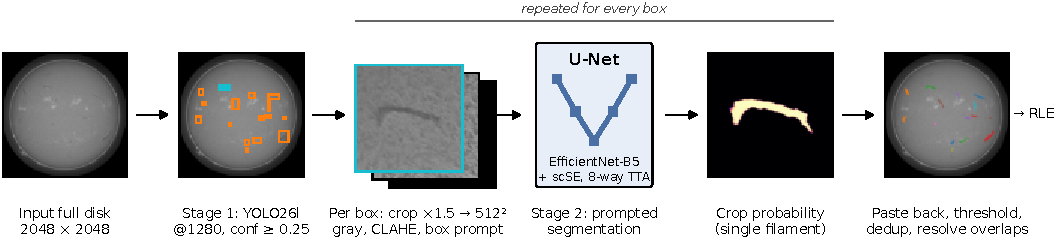
\includegraphics[width=\textwidth]{pipeline.pdf}
    \caption{Final inference pipeline on a validation image. Stage~1: a YOLO26l detector proposes one box per filament. Stage~2: each box becomes a three-channel square crop (grayscale, CLAHE, box prompt; one box highlighted), a U-Net segments the prompted filament, and the crop probabilities are pasted back, thresholded, deduplicated and made non-overlapping (masks dilated for visibility).}
    \label{fig:pipeline}
\end{figure*}

\subsection{Data and Validation Split}
The training set contains 707 full-disk images with 1,154 annotator records; many images were labelled independently by two or three annotators. We hold out 15\% of the \emph{physical} images (seed 42) as a fixed validation split, keeping all records of an image on one side: 601 images (984 records, 6,941 filaments) for training and 106 images (170 records, 1,258 filaments) for validation. Every model selection and comparison in this report uses this split.

\subsection{Two-Stage Pipeline}
Figure~\ref{fig:pipeline} shows the pipeline. Separating detection from segmentation lets the U-Net work on small, high-resolution crops: 97\% of validation crops are \emph{upsampled} to the network input, so thin filaments are never shrunk.

    \textbf{Stage 1: Detection.} A single-class YOLO26l detector \cite{jocher2026ultralyticsyolo26unifiedrealtime}, initialized from COCO weights, is fine-tuned on full images at $1280\times1280$\,px. Each annotator record is a separate training sample whose targets are that annotator's filament boxes. We train for up to 200 epochs (early-stopping patience 25) at batch size 8 with mosaic and horizontal and vertical flips, and keep the checkpoint with the best validation mAP. At inference, boxes pass non-maximum suppression (NMS) at IoU 0.20 and are kept if their confidence is $\geq 0.25$ (at most 100 per image).

    \textbf{Stage 2: Prompted Segmentation.} Each box is expanded to a square crop of $1.5\times$ its longer side (zero-padded at the image edge) and resized to $512\times512$. The crop has three channels: the grayscale image, a CLAHE-enhanced copy (clip limit 1.5, $8\times8$ tiles) \cite{zuiderveld1994clahe}, and a binary rectangle marking the box, which tells the network \emph{which} filament to segment when a crop contains several. The network is a U-Net \cite{ronneberger2015unet} with an ImageNet-pretrained EfficientNet-B5 encoder \cite{tan2019efficientnet} and concurrent spatial and channel squeeze-and-excitation \cite{roy2018scse} in the decoder, built with segmentation\_models\_pytorch \cite{smp}.

    Training crops come from annotated filaments: the ground-truth box is shifted by up to $\pm20\%$ of its size and expanded by a random factor in $[1.25, 1.75]$, so the network sees the imperfect crops it will meet at test time, followed by random flips and $90^\circ$ rotations. We add 1,270 \emph{hard negatives}, false-positive detector boxes on training images, with empty targets, so the U-Net learns to return nothing for spurious boxes. The loss is $0.25\cdot\mathrm{BCE} + 0.75\cdot$ focal Tversky \cite{salehi2017tversky,abraham2019focal} with $\alpha=\beta=0.5$ and $\gamma=0.75$, optimized with AdamW \cite{loshchilov2019adamw} (learning rate $3\cdot10^{-4}$, weight decay $10^{-4}$, two warm-up epochs then cosine decay) at batch size 16 with mixed precision. After each epoch the full pipeline runs on the validation split and the checkpoint with the best official PQ is kept (epoch 6), so selection directly penalizes false positives.

    \textbf{Post-processing.} The U-Net output is averaged over eight views of each crop (four rotations, each with and without a horizontal flip), pasted back at full resolution, thresholded at 0.45, and discarded below 20 pixels. Each instance is scored by detector confidence $\times$ mean mask probability; instances are visited in score order and dropped if they overlap a kept mask with IoU $\geq 0.5$ or containment $\geq 0.8$. Contested pixels go to the instance with the highest probability $\times$ score, which guarantees non-overlapping masks.

\subsection{From Baselines to the Final Model}
    \textbf{Baselines.} We first trained seven YOLO26 detectors (sizes n to x, at 1024 or 1280\,px) and the B5 U-Net. The best single pair, YOLO26x with the B5 U-Net, scored 0.36 on the public leaderboard.

    \textbf{Ensemble.} Boxes from several detectors are combined with weighted box fusion \cite{solovyev2021wbf}: boxes are clustered at IoU 0.40, coordinates are confidence-weighted averages, and a cluster's score is the fraction of detector views that found it, so a filament found by most detectors outranks one found by a single detector. Running every detector also on horizontally and vertically flipped images triples the views, and the masks of several U-Nets are averaged before thresholding. Eight detectors (the seven baselines plus a YOLO11m) $\times$ three views with three U-Nets scored 0.39 publicly.

    \textbf{Teacher and Students.} To keep the ensemble's accuracy at a fraction of the cost, this 24-view ensemble served as a \emph{teacher} and labelled 1,000 unlabeled GONG H-$\alpha$ images with 4,840 boxes (fused score $\geq 0.3$). Seven \emph{student} detectors were trained on the 984 competition records plus these images with the recipe above \cite{lee2013pseudo,xie2020noisystudent}. The students are stronger single models than their predecessors. Adding them and two more detectors to the ensemble (17 detectors, 51 views, three U-Nets) scored 0.40 publicly but only tied it locally, and requires 20 checkpoints (383M parameters) and 51 detector passes per image.

    \textbf{Final Solution.} We keep one student, YOLO26l (26.2M parameters), and one U-Net (31.3M) with 8-way test-time augmentation (TTA). The U-Net is trained on competition data only; U-Nets trained on teacher-drawn pseudo-masks did not improve mask quality.

\subsection{External Data}
The organizers permit unlabeled GONG H-$\alpha$ observations. The 1,000 pseudo-labelled frames come from the public GONG archive, the same product as the competition images, with stations sampled uniformly over the six sites and years following the training distribution; every day within $\pm1$ day of a training or test image was excluded. Each frame was also checked against all 180 test images by timestamp ($\pm1$\,h), file hash, and normalized correlation of fine image structure, which detects a re-encoded copy of a frame; none was flagged. Section~\ref{sec:evaluation} shows that the final detector performs equally well without this data.


% ==================================== %
%              EVALUATION              %
% ==================================== %
\section{Evaluation}\label{sec:evaluation}
\subsection{Protocol}
All scores are official PQ on the 106 validation images, computed against each annotator record separately with counts pooled, exactly as in the organizers' evaluation code; their code gives the same value on our predictions to six decimals (0.466609). Every comparison is \emph{paired}: both pipelines run on identical images, and we report the PQ difference $\Delta$ with a 95\% bootstrap interval over images. We call a change a gain or a loss only when its interval excludes zero. With a bootstrap standard deviation of 0.013 for a single pipeline, differences under about 0.01 are usually not resolved. The public leaderboard tracks local PQ at about $0.82\times$ and shows two decimals, so it cannot separate such pipelines either.

\begin{table}[t]
  \caption{Main results (validation PQ; TP/FP/FN pooled over annotator records).}
  \label{tab:main}
  \footnotesize
  \setlength{\tabcolsep}{2.5pt}
  \begin{tabular}{@{}lrrrrrrr@{}}
    \toprule
    Pipeline & Views & Params & PQ & TP & FP & FN & Public \\
    \midrule
    Baseline (26x + B5) & 1 & 90M & .427 & 783 & 464 & 475 & .36 \\
    Ensemble, 8 det. & 24 & 253M & .474 & 834 & 333 & 424 & .39 \\
    Ensemble, 17 det. & 51 & 383M & .474 & 823 & 314 & 435 & .40 \\
    \textbf{Final} (l\_ps) & 1 & 57.5M & .467 & 828 & 360 & 430 & .39 \\
    Final, no ext.\ data (l\_pl) & 1 & 57.5M & .466 & 808 & 317 & 450 & .38 \\
    \bottomrule
  \end{tabular}
\end{table}

\subsection{Main Results}
Table~\ref{tab:main} compares the pipelines. The final pipeline improves on the baseline by $\Delta = +0.039$ [$+0.027$, $+0.052$], finding 45 more filaments with 104 fewer false positives, and is statistically tied with the 51-view ensemble ($-0.008$ [$-0.018$, $+0.002$]) and the 24-view ensemble ($-0.007$ [$-0.017$, $+0.004$]). End to end, including image loading, it takes 0.44\,s per image on an A100 and 1.57\,s on a T4, under five minutes for the 180 test images on a free GPU. We chose it over the 0.40 ensemble because their one-step public difference is within rounding and our local intervals.

\begin{table}[t]
  \caption{Ablation. Top: the detector, each row adding one change to the row above (same U-Net and TTA). Bottom: Stage~2 changes to the final pipeline. $\Delta$ with 95\% paired CI.}
  \label{tab:ablation}
  \footnotesize
  \setlength{\tabcolsep}{3pt}
  \begin{tabular}{@{}lccl@{}}
    \toprule
    Detector (YOLO26l) & mAP & PQ & $\Delta$ [95\% CI] \\
    \midrule
    Baseline recipe & .387 & .436 & -- \\
    + vertical flips, batch 8 (l\_pl) & .409 & .466 & +.030 [+.015, +.046] \\
    + pseudo-labels (l\_ps, final) & .417 & .467 & +.001 [$-$.014, +.014] \\
    \midrule
    Stage 2, vs.\ final & & PQ & $\Delta$ [95\% CI] \\
    \midrule
    No test-time augmentation & & .463 & $-$.004 [$-$.006, $-$.001] \\
    Baseline U-Net & & .457 & $-$.010 [$-$.017, $-$.004] \\
    \bottomrule
  \end{tabular}
\end{table}

\subsection{Ablation}
Table~\ref{tab:ablation} separates the changes between the baseline and final detectors. Retraining the same YOLO26l with vertical flips (solar images have no preferred orientation) and a fixed batch size of 8 (automatic selection had chosen batches too small for stable batch normalization) gains 0.030 PQ. Adding the pseudo-labelled images then raises mAP50-95 from 0.409 to 0.417 but leaves PQ unchanged. The teacher's knowledge reaches the student, but its benefit is not measurable after Stage~2, likely because the pseudo-labels mostly add confident, easy filaments, while PQ is limited by faint filaments and mask boundaries (Section~\ref{sec:errors}). In Stage~2, the symmetric-Tversky U-Net selected by pipeline PQ gains 0.010 over the baseline U-Net, and TTA adds 0.004.

\begin{table}[t]
  \caption{Inference hyperparameters of the final pipeline, one at a time (chosen value in bold; $^\dagger$\,loss, CI excludes zero).}
  \label{tab:hyper}
  \small
  \setlength{\tabcolsep}{3.5pt}
  \begin{tabular}{@{}l*{6}{c}@{}}
    \toprule
    Box NMS IoU & 0.10 & \textbf{0.20} & 0.30 & 0.50 & 0.70 & none \\
    \quad PQ & .466 & \textbf{.467} & .467 & .467 & .467 & .468 \\
    Inference size (px) & 1024 & \textbf{1280} & 1536 & 2048 & & \\
    \quad PQ & .465 & \textbf{.467} & .453$^\dagger$ & .443$^\dagger$ & & \\
    Crop expansion & 1.25 & \textbf{1.50} & 1.75 & 2.00 & & \\
    \quad PQ & .463$^\dagger$ & \textbf{.467} & .466 & .462$^\dagger$ & & \\
    \quad Coverable filaments & 81.4\% & \textbf{82.9\%} & 83.8\% & 84.9\% & & \\
    \quad Crops with $\geq$2 filaments & 6.2\% & \textbf{9.5\%} & 11.9\% & 14.9\% & & \\
    Mask threshold & 0.35 & \textbf{0.45} & 0.55 & & & \\
    \quad PQ & .466 & \textbf{.467} & .463$^\dagger$ & & & \\
    \bottomrule
  \end{tabular}
\end{table}

\begin{figure}[t]
    \centering
    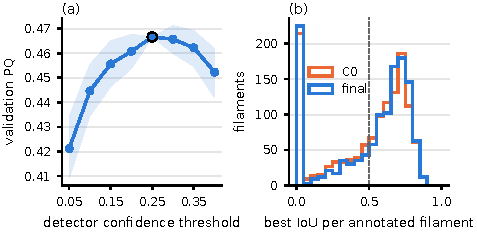
\includegraphics[width=\columnwidth]{tuning.pdf}
    \caption{(a) Validation PQ against the detector confidence threshold; the band is the 95\% paired interval relative to the chosen 0.25. (b) Best IoU reached by any prediction for each of the 1,258 annotated filaments, final pipeline vs.\ baseline; a filament counts as found above 0.5 (dashed).}
    \label{fig:tuning}
\end{figure}

\subsection{Hyperparameter Selection}
Each inference setting was varied on the final pipeline with everything else fixed (Table~\ref{tab:hyper}, Figure~\ref{fig:tuning}). The settings were chosen on the reported validation split; in our earlier measurements, tuning one threshold this way inflated validation PQ by about 0.003.

    \textbf{Confidence Threshold.} This is the most important setting. At 0.05 the detector proposes 1,270 boxes and the pipeline finds 99 more filaments but produces 475 more false positives, losing 0.045 PQ. From 0.20 to 0.35, PQ stays within 0.006 of 0.25, and it drops at 0.40 as true positives are lost. We chose 0.25, the middle of this plateau, so the setting is robust to small shifts in detector confidence on the test set.

    \textbf{NMS IoU.} PQ does not depend on it: every value from 0.10 to 0.70, and YOLO26's NMS-free output, lie within 0.0013, because overlapping boxes produce near-identical masks that the mask deduplication removes. A low IoU of 0.20 simply avoids segmenting duplicates (769 boxes vs.\ 829 at 0.70).

    \textbf{Image Size.} The detector is best at its training size: at inference, 1024\,px ties 1280\,px, while 1536 and 2048\,px lose 0.014 and 0.023. For training, moving YOLO26s from 1024 to 1280\,px gained 0.010 PQ, whereas 1536\,px gave a non-significant $+0.005$ [$-0.009$, $+0.018$] at $1.44\times$ the pixels, so we kept 1280.

    \textbf{Crop Expansion.} We call a filament \emph{coverable} when one crop holds more than half its pixels, the minimum needed to reach IoU 0.5. Widening crops from 1.5 to 2.0 raises coverage by only 2 points, whereas lowering the confidence threshold from 0.25 to 0.05 raises it by 11, so coverage is set by the detector, not the crop. Since every crop is resized to 512\,px, wider crops cost no compute, but they cost resolution (25\% fewer pixels across the filament at 2.0) and add ambiguity (crops with two or more filaments rise from 9.5\% to 14.9\%). Both 1.25 and 2.0 lose PQ; 1.5, the middle of the training range, is best.

\begin{figure*}[t]
    \centering
    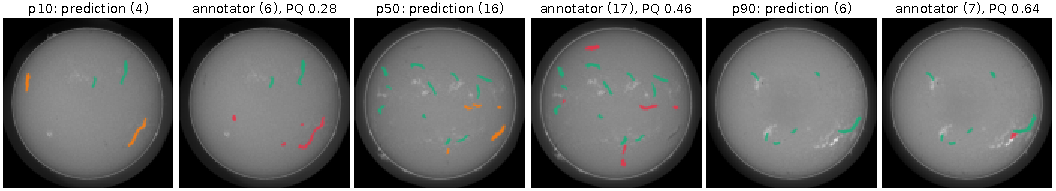
\includegraphics[width=\textwidth]{examples.pdf}
    \caption{Final-pipeline predictions on validation images at the 10th, 50th and 90th percentile of per-image PQ, each next to the annotator with the most filaments. Green: matched (IoU $>0.5$); orange: unmatched prediction; red: missed annotation. Masks dilated for visibility.}
    \label{fig:examples}
\end{figure*}

\begin{figure*}[t]
    \centering
    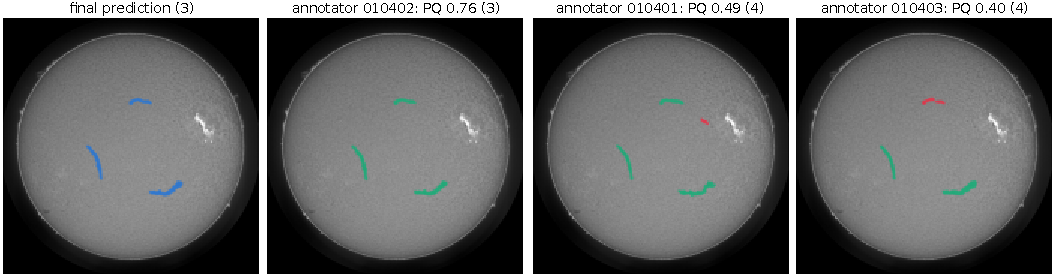
\includegraphics[width=\textwidth]{annotators.pdf}
    \caption{One prediction, three annotators. The same three predicted masks (left) score PQ 0.76, 0.49 and 0.40 against the three annotators of this validation image. Annotator 010401 adds a small filament and draws boundaries differently (mean matched IoU 0.58 vs.\ 0.76); annotator 010403 splits the top filament in two, turning one correct mask into one false positive and two misses. Green: matched (IoU $>0.5$); red: missed.}
    \label{fig:annotators}
\end{figure*}

\begin{figure}[b]
    \centering
    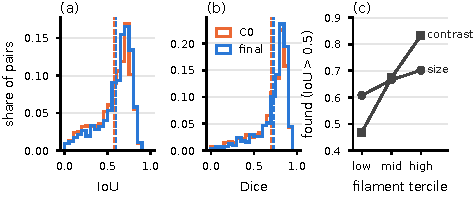
\includegraphics[width=\columnwidth]{distributions.pdf}
    \caption{(a, b) IoU and Dice of all overlapping prediction--annotation pairs (dashed: means). (c) Filaments found (best IoU $>0.5$) by tercile of area and of contrast (darkness against a 15-px band around the filament).}
    \label{fig:distributions}
\end{figure}

\subsection{Annotator Disagreement}
    The largest source of variation in PQ is the annotator rather than the model. On the 40 validation images labelled by two or three annotators, the PQ of the \emph{same} prediction differs between annotators by 0.19 on average (median 0.15, maximum 0.57). Annotators disagree both on \emph{which} structures are filaments and on \emph{how} to draw them: only 53\% of one annotator's filaments are matched (IoU $>0.5$) by another's, and the union of an image's annotators holds 11.2 filaments versus 6.8 per annotator (Figure~\ref{fig:annotators}). Over the split, PQ against individual annotators ranges from 0.36 to 0.58, while two annotators scored against each other reach only 0.34, so the pipeline agrees with each annotator more than annotators agree with each other. Differences of about 0.01 between pipelines are therefore below what this data can resolve. Suppressing low-confidence filaments to match the sparsest annotators would raise PQ while contradicting the organizers' request to detect every filament, so we did not tune for it.

\subsection{Error Analysis}\label{sec:errors}
    Figure~\ref{fig:tuning}b shows where the gain over the baseline comes from. The share of filaments the pipeline never touches (IoU $<0.05$) stays at about 18\%: the detector does not propose them at any setting we use. The improvement comes from filaments that were found but drawn too loosely and now pass IoU 0.5 (65.8\% matched vs.\ 62.2\%), and from 22\% fewer false positives. Matched masks reach a mean IoU of 0.69 (Dice 0.81). Over every overlapping prediction--annotation pair (Figure~\ref{fig:distributions}a,b), the organizers' code gives a mean IoU of 0.60 and Dice of 0.73, against 0.57 and 0.70 for the baseline. Fragmentation (one filament split into several predictions) is 3.5\% and over-merging (several filaments in one prediction) 2.0\%, against 3.7\% and 2.9\%. Figure~\ref{fig:examples} shows typical failures. At the 10th percentile, the pipeline segments a long filament that this annotator traced as several pieces, and finds two filaments the annotator did not mark. At the median, most misses are small, faint filaments; size and contrast act almost independently (Figure~\ref{fig:distributions}c), and the faintest third of filaments is found 47\% of the time against 83\% for the highest-contrast third.

\section{Limitations and Future Work}
The detector never proposes about 18\% of annotated filaments, mostly small and faint ones, and matched-mask IoU stays near 0.69 under every loss and U-Net we tried, suggesting a ceiling set by how annotators trace boundaries. A detector retrained on CLAHE-enhanced inputs gained mAP (0.425 vs.\ 0.417) but not PQ ($-0.011$ [$-0.023$, $0.000$]), so future work should target recall with data beyond the 8-bit images, such as the original FITS observations.

% ==================================== %
%            ACKNOWLEDGMENT            %
% ==================================== %
\section{Acknowledgment}\label{sec:acknowledgment}
    % Do not change
    The organization of the Filament Segmentation Challenge 2026 is partially supported by the U.S. National Science Foundation (NSF) under Grant No. 2209912 and 2433781, directorate for Computer and Information Science and Engineering (CSE), and Office of Advanced Cyberinfrastructure (OAC), and Grant No. 2511630, AST Division Of Astronomical Sciences and MPS Directorate for Mathematical and Physical Sciences.

    The Filament Segmentation Challenge 2026 is sponsored by the U.S. National Science Foundation (NSF) National Solar Observatory (NSO).

    This work utilizes GONG data obtained by the NSO Integrated Synoptic Program, managed by the National Solar Observatory, which is operated by the Association of Universities for Research in Astronomy (AURA), Inc. under a cooperative agreement with the National Science Foundation and with contribution from the National Oceanic and Atmospheric Administration. The GONG network of instruments is hosted by the Big Bear Solar Observatory, High Altitude Observatory, Learmonth Solar Observatory, Udaipur Solar Observatory, Instituto de Astrofísica de Canarias, and Cerro Tololo Interamerican Observatory.

    We used Claude Code throughout this project to help write and run experiment code, create charts and figures, and help revise this report. All design decisions, experiments, and results were reviewed by the author, who takes full responsibility for the work and its scientific accuracy.

\bibliographystyle{ACM-Reference-Format}
\bibliography{main}

\end{document}
